% Chapter 1

\chapter{Absolute power calibration} % Main chapter title
\label{Chapter5} % For referencing the chapter elsewhere, use \ref{Chapter1} 
This chapter describe the absolute power calibration procedure of KAGRA photon calibrator.
The systematic error of the absolute power is most largest in LIGO.
They measure the laser power with integrating sphere and InGaAs photodetector because displacement of mirror corresponds to laser power. 
The absolute power injected to the ETM can be obtained as average of input power at Tx module and the output power at Rx module as follows:
\begin{equation}
P=\frac{P_{TxPD}+P_{RxPD}}{2}=\frac{1+e}{2e}P_{RxPD},
\end{equation}
where $P_{TxPD}$ and $P_{RxPD}$ are the measured power of the transmitter module photo detector(TxPD) and the receiver module photodetector (RxPD), and $e=P_{TxPD}/P_{RxPD}$ is optical efficiency.
Therefore, $P_{TxPD}$ and $P_{RxPD}$ limit the calibration accuracy of the absolute displacement of the mirror.
To calibrate $P_{TxPD}$ and $P_{RxPD}$, we employ the working standard (WS) and the gold standard (GS). 

The WS of KAGRA (WSK) is the combination of integrating sphere and InGaAs photo detector (see Fig.~\ref{fig:KWS}), which is calibrated against GS of LIGO (GSL) in LHO lab as calibrated by NIST. LIGO also make working standards for LHO and LLO as shown in Fig~\ref{fig:GS_WS}.
The ratio of measured voltage of WS and GS detectors are obtained as
\begin{equation}
\frac{V_{WSK}}{V_{GSL}}.
\end{equation}
We can calibrate the response of WS using GS through this equation.

We will also use the WSK to calibrate the TxPD and RxPD, which are inside the Tx module and Rx module of Pcal, respectively. We will measure the ratio of voltage of TxPD and RxPD as follows
\begin{equation}
\frac{V_{TxPD}}{V_{KWS}}.
\end{equation}

Finally,  we obtain the calibration power $P_{GW}$ using the power standard laser in NIST.
Then, we can get the calibrated $P_{TxPD}$ and $P_{RxPD}$ as follows:

\begin{eqnarray}
P_{TxPD}=\frac{V_{TxPD}}{V_{KWS}}\frac{V_{WSK}}{V_{GSL}}P_{GS}, \\
P_{RxPD}=\frac{V_{RxPD}}{V_{KWS}}\frac{V_{WSK}}{V_{GSL}}P_{GS}
\end{eqnarray}

\begin{figure}
\begin{center}
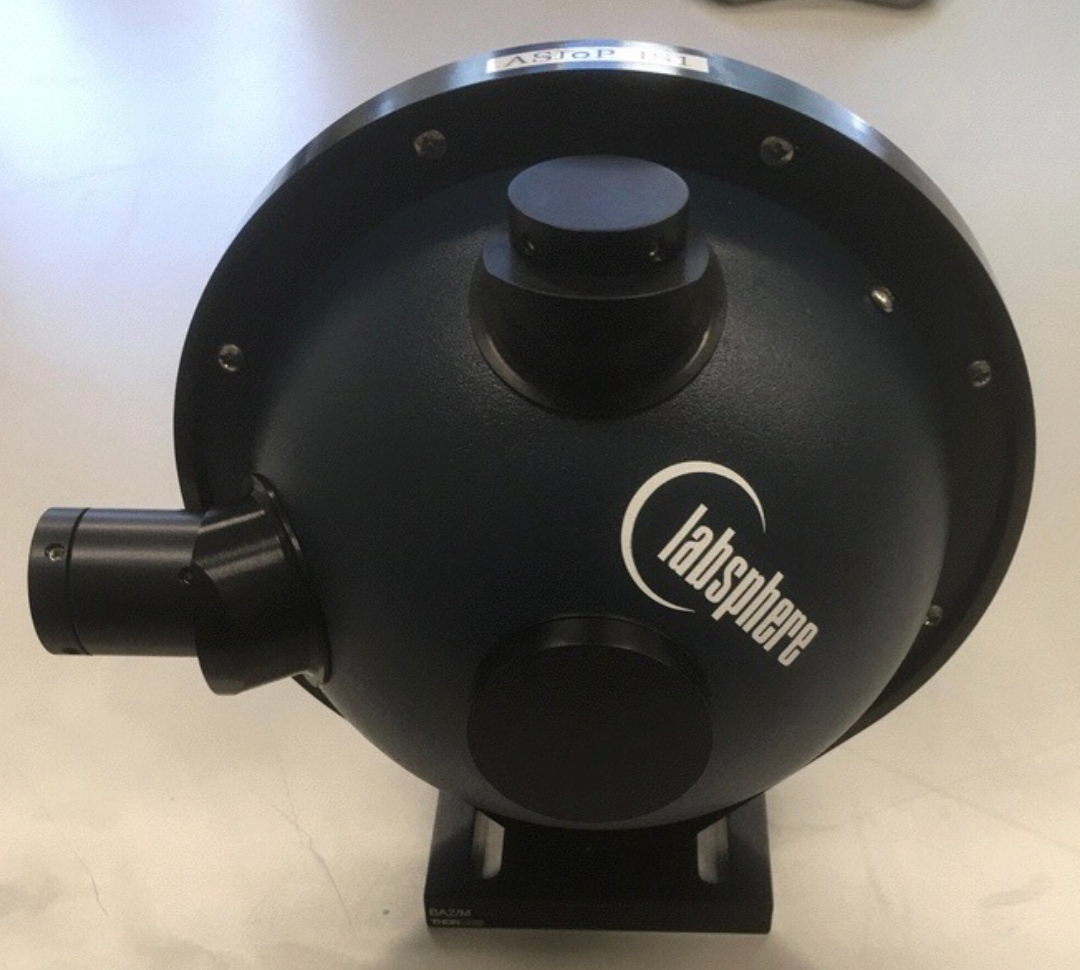
\includegraphics[width=14cm]{Figures/KWS.eps}
\caption{KAGRA working standard.} 
\label{fig:KWS} 
\end{center}
\end{figure}

\begin{figure}
\begin{center}
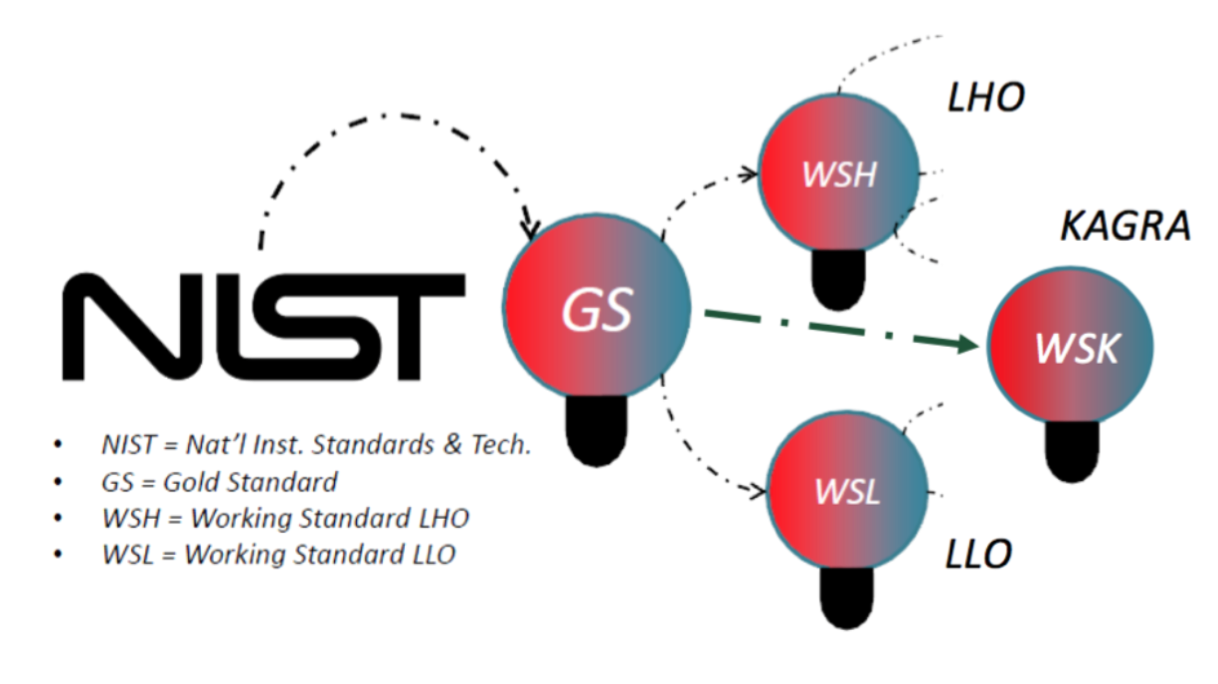
\includegraphics[width=14cm]{Figures/GS_WS.eps}
\caption{comparison with GS and WS.} 
\label{fig:GS_WS} 
\end{center}
\end{figure}

\section{Calibration in LHO}
%\begin{figure}
%\begin{center}
%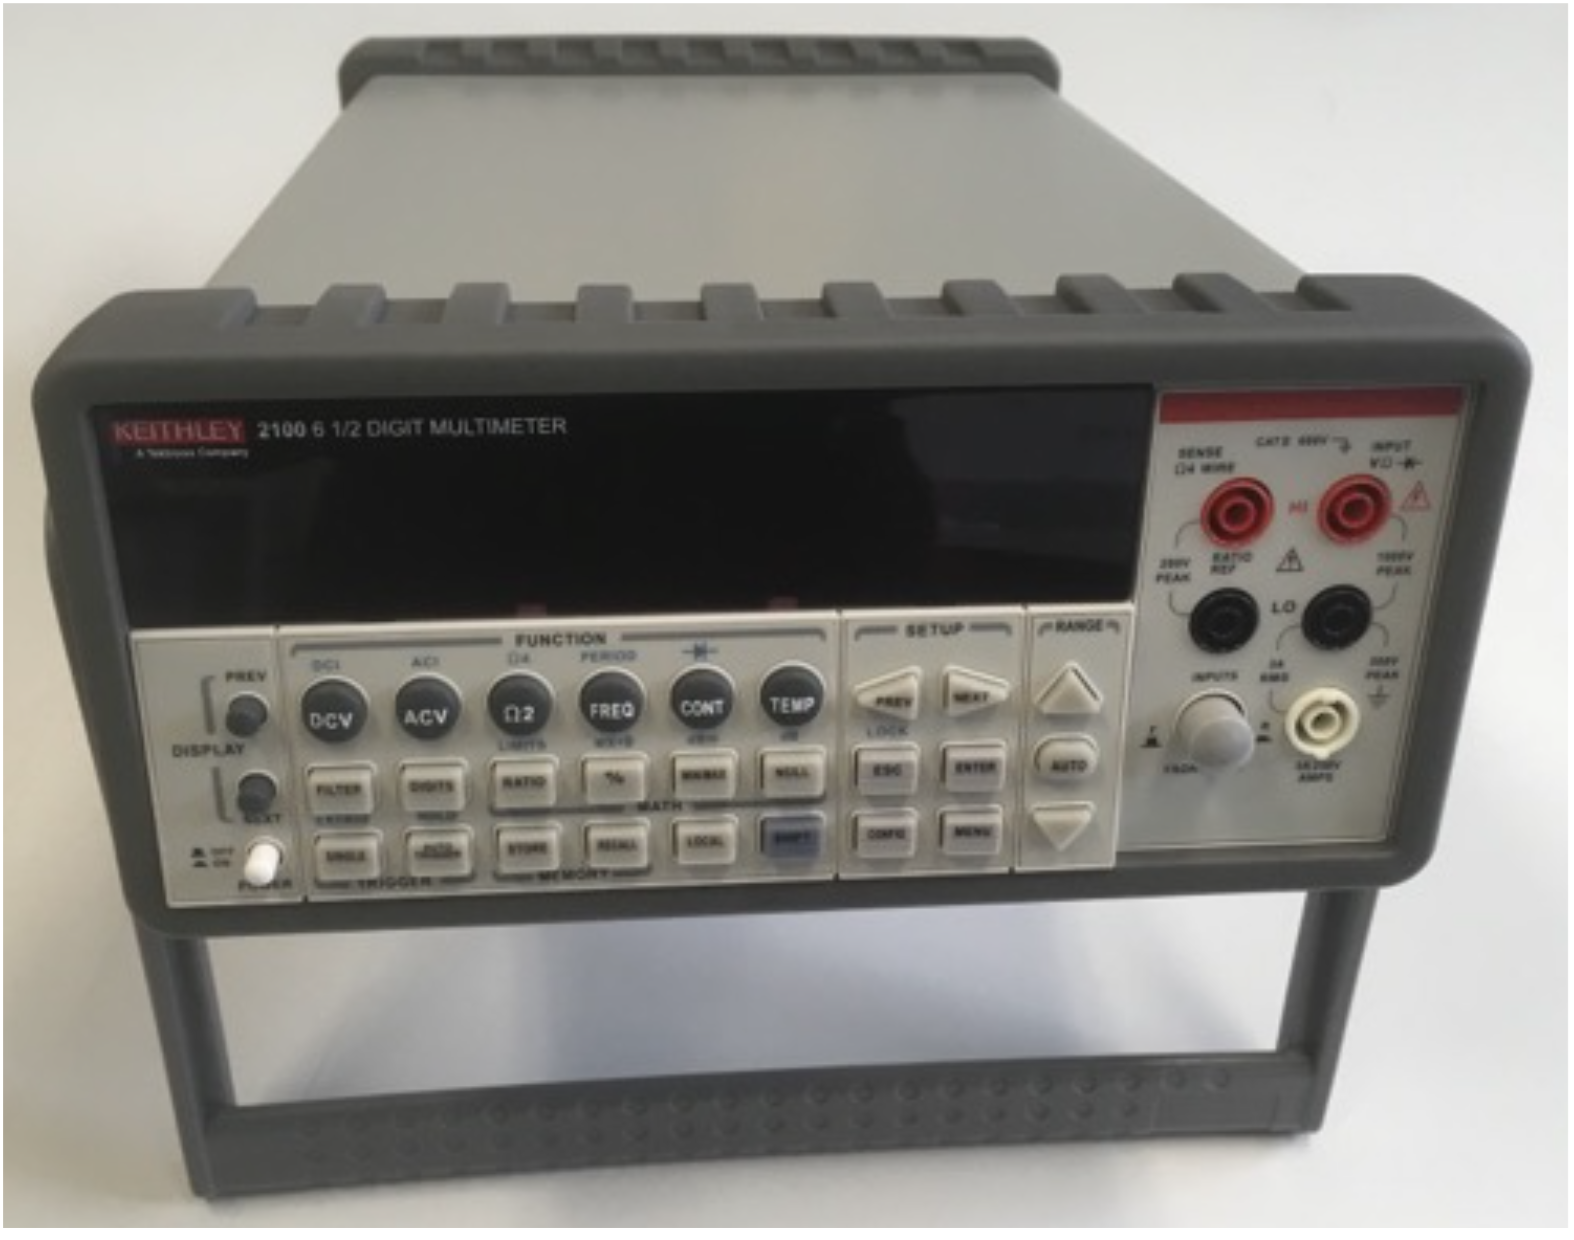
\includegraphics[width=14cm]{Figures/Keithlay.eps}
%\caption{.} 
%\label{fig:Keithlay} 
%\end{center}
%\end{figure}
%-------------------------------
\section{Calibration in End-station}
%-------------------------------
%\section{Gold standard}
%-------------------------------
%\section{Working standard}
\section{Summary}








